
\chapter{Design overview and system design}
Het systeem is opgedeeld in vier blokken:
\begin{itemize}
\item De main controller
\item De DCF controller
\item De LCD controller
\item Het alarm
\end{itemize}

\noindent In figuur \ref{fig:blokdiagram} is te zien welke ingangs- en uitgangssignalen het systeem in en uit gaan en hoe de blokken elkaar aansturen.

\begin{figure}[h!]
\center
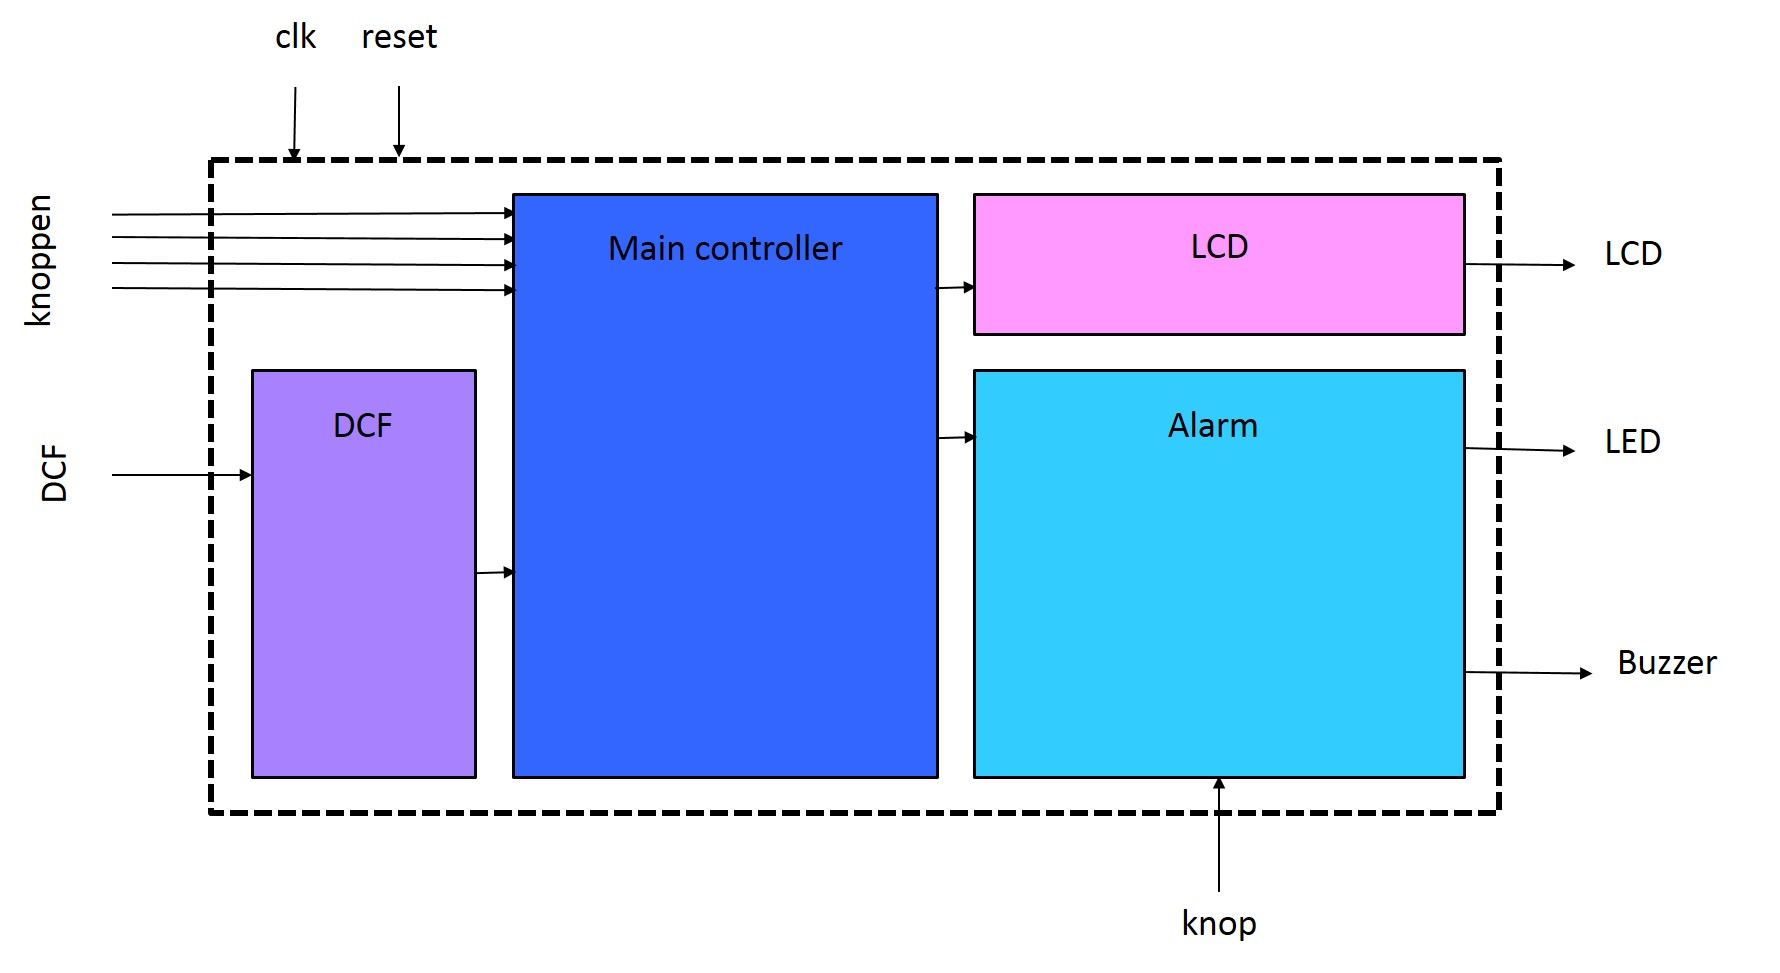
\includegraphics[width=13cm]{figure/blokdiagram}
\caption{Blokdiagram van het gehele systeem}
\label{fig:blokdiagram}
\end{figure}

\noindent De main controller bestuurt het hele systeem. De alarmtijd kan ingesteld worden en de alarmtijd wordt met de actuele tijd vergeleken.\\
De DCF controller vangt het DCF signaal op en zet het om naar een bitvector met datum, uren en minuten. En er wordt een kloksignaal van 1 Hz gegenereerd.\\
De LCD controller zorgt dat de datum, tijd, ingestelde alarmtijd en de veranderingen in het menu op de LCD zichtbaar zijn. Er wordt een LCD scherm gebruikt waar de pixels afzonderlijk van elkaar aangestuurd worden. Tussen de chip en het scherm zit nog een microcontroller, waarin de karakters zijn opgeslagen, dit zou namelijk te groot zijn om op de chip te regelen.\\
Het alarm zorgt ervoor dat een PWM-signaal gegenereerd wordt wat naar een LED gaat.